%This file will be included in the ThesisMain Document as the experimentation
%section.

%Author: James Kelly
%Last Modified: 11-12-08

\begin{center}
\section{Discussion and Results}
\end{center}

The fundamental motivation for this experimentation was first and foremost to quantify the thermal sink capacity of a bulk aggregate. Additionally, results should demonstrate that a mass of such material can and will remove a measurable amount of thermal energy from a thermally charged flow. Any result short of this hypothesis would effectively render the implementation of aggregate material ineffective as a solution to thermally charged stormwater discharge. Some material comes close to being thermally inert with respect to removing adequate amounts of thermal energy from a hydraulic flow. However, most material has demonstated some capacity to sink a thermally charged flow.
 
It is especially noteworthy in the case of most of the tested materials, given the relatively small thermal heat capacity and thermal conductivities, that the quantity and rates of heat were observed. The experiment was conceived on the hypothesis that aggregate materials were incorrectly assumed to have significant thermal sinking effects. Furthermore, some samples offer significant potential to relieve thermal duress under flow in severe scenarios, if implemented properly. It is therefore the goal of this discussion to consider the data and provide a foundation for further research and insight into using un-consolidated materials - of any form - to thermally sink a hydraulic discharge.

\subsection{Aggregate Parameters}

Several metrics are used in the performance analyses and ranking of the test materials. Bearing in mind that some of the materials were included in the experimentation strictly to diversify experimental results, several general conclusions can be stated with regard to completely practical materials. This section discusses these metrics and explains their role in the evaluation of an un-consolidated material's thermal sink performance.

Specific intrinsic parameters were identified and used to guide experimentation. Additionally, several environmental variables were also identified and used likewise. The choice of these parameters was based on the expectation that a respective variation would have a measurable effect on the thermal sink capacity of the sample aggregate. Several of these parameters were not directly measured or included in the current analysis primarily because they exceeded the intended scope of the experiment and available resources. However, results from theoretical renderings indicate some of these untested parameters may play an important role in an aggregate's thermal response. Some of these parameters include porosity, fineness modulus, isotropy, Mohs hardness and cobble geometry. For the purposes of this discussion, such parameters have been ruled as having only peripheral effects compared to more dominant parameters such as cobble size, bulk density and composition, and are consequently not part of this analysis. Continuing experimentation should investigate possible thermal relationships with these characteristics. 

Parameters that were isolated and studied for their contribution toward any sort of thermal response in a sample are listed in Table (\ref{matrix}). In considering material based characteristics, all tested aggregates share a comparatively narrow range of thermal properties given that they are all some sort of rock \citep{heatxfer}. Material is the single most dominant characteristic with respect to heat capacity $C_{R}$ and thermal conductivity $k$. That is to say that if a material with twice the heat capacity and thermal conductivity is used, a similar change in cobble size will have much less of an effect. This result was confirmed with the testing of both glass and steel balls in comparison to aggregate materials. In generalizing the results beyond aggregates, it is necessary to bear this in mind. However, in the regime of aggregate materials, the dominant variable that emerges is cobble size, because the materials are all quite similar with respect to $c_{R}$ and $k$. 

\begin{table}[t] 
\centering                           
\caption[Thermal Sink Parameters]{Thermal Sink Parameters: These intrinsic parameters were isolated and used to direct experimentation and theory and are listed in their order of their measured contribution to thermal sink capacity.\label{matrix}} 
\begin{tabular}{l l}           
\\[1ex] 
\hline\hline             
Intrinsic Parameters
\\
\hline 
\\
Material\\
Characteristic Radius\\
Mass\\
Packing Fraction\\
\\
\hline\hline
Systemic Parameters\\
\hline
\\
Flow Rate\\
Initial Flow Temperature\\
\\
\hline\hline
\end{tabular}
\label{tab:matrix}
\end{table}

Beyond using various types of aggregate to acheive a range of outcomes, reservoir temperature was varied slightly in addition to various flow rates. A variance in reservoir temperature did not change aggregate performance, but merely provided a basis for a thermal scaling of results. A ranking of aggregate thermal performance should be the same under any similar thermal potential and the total energy removed should also be the same. The time over which that energy is transferred to the aggregate will be exponentially slower with a decrease in the reservoir temperature. 

A variance in flow rate will naturally change the rate at which thermal energy is available for transfer. However, a varying flow rate also will affect the contact area between the flow and the aggregate surface area. This is true up to the point where the volume of fluid delivered to the aggregate in a period of time completely fills the interstitial space. At this point, the gravitationally driven flow will provide backpressure, and the aggregate will impose a different flow resistance. It is unknown if this scenario would present a different thermal transfer regime, as the available flow rates were always accommodated by the samples. The actual fraction of interstitial volume displaced by a known flow depends on several aggregate parameters, including geometry, packing fraction, porosity and surface interactions and overall fineness or cobble count. The fraction of interstitial volume displaced by flow can be estimated as follows:

\begin{equation}\label{flowDisp}
 Interstitial\:Flow\:Volume\:=\frac{I_{V}-\nu_{W}(t)}{I_{V}}
\end{equation}
\begin{equation}\label{sa}
Bulk\:Surface\:Area\:\approx\;4\pi R_{s}^{2}\;n\;M_{s}\left[\frac{nI_{V}}{V}\right]
\end{equation}
\begin{equation}\label{contact}
 Contact\:Area\;\approx\frac{Interstitial\:Flow\:Volume}{I_{V}}\:(Bulk\:Surface\:Area)
\end{equation}

In Equation \ref{sa}, the right hand term is a ratio that can be used to estimate the obliqueness of cobble geometry by accounting for the amount of interstitial space per cobble. Omitting this term would estimate a bulk surface area by assuming the cobbles are spherical. In Equation \ref{contact} the contact area is estimated as a real surface area, or by only considering the fractional part, as a ratio of the available surface area. This Equation includes several assumptions including the contact area between cobbles being negligible. Additionally, concavity of surfaces and porosity are not considered. 

\begin{table}[h] 
\centering                           
\caption[Contact Area Ratios]{Estimated contact area is expressed as a ratio with the available bulk contact area and is computed for each flow rate used in the experiment.\label{contactT}} 
\begin{tabular}{c c c}           
\\[1ex] 
\hline\hline
\\             
Flow Description & Flow Rate $\frac{L}{s}$ & Est Contact Area Ratio\\
\\
\hline
\\
Low & 0.20-0.30 & 0.18\\
Med & 0.35-0.45 & 0.23\\
High & 0.50-0.55 & 0.31\\
\\
\hline\hline
\end{tabular}
\label{tab:matrix}
\end{table}

In considering the flow through the vessel, we have not assumed any preferential flow patterns. The inflow has been observed to be very turbulent and the aggregate is randomly arranged such that there is little reason to suspect a highly preferential flow. However, larger cobbles such as QM5 and S2, and the steel and glass balls, have been thought to encourage more preferential flows, especially when noting their respective packing arrangements in the 4'' vessel. Specifically, a more voluminous flow along the walls of the vessel would bypass, to some degree, the main bulk of the sample. 

\subsection{Concepts of Thermal Sink Performance Metrics}

In reviewing the various parameters and related measures for rating the thermal sink performance of a particular un-consolidated material, it is pertinent to discuss how parameters affect or are affected by specific outcomes in the models and methods prescribed thus far. The following curves are plotted using the thermal potential model in Equation (\ref{rcNew}). In Figure (\ref{sinkComp1}) two samples with different specific heats and different thermal conductivities have been modeled. The ideal material possesses a thermal moment of $10\:\frac{kg}{m\bullet s}$ and the less responsive material possesses a thermal moment of $7\:\frac{kg}{m\bullet s}$. The ideal material has a much higher specific heat capacity and thermal conductivity, which is manifested in a steep ramp to its maximum J/K/Kg value. The ultimate amplitude of each curve is a direct result of the materials specific heat capacity, and the time until the curve reaches that level is a function of the thermal conductivity. The thermal diffusivity is not directly calculable from this information, as mass and bulk density directly affect it's value. If the slow response material were sufficiently lighter and less dense than the ideal sink material, the thermal diffusivity value could rate it higher.

\begin{figure}
 \centering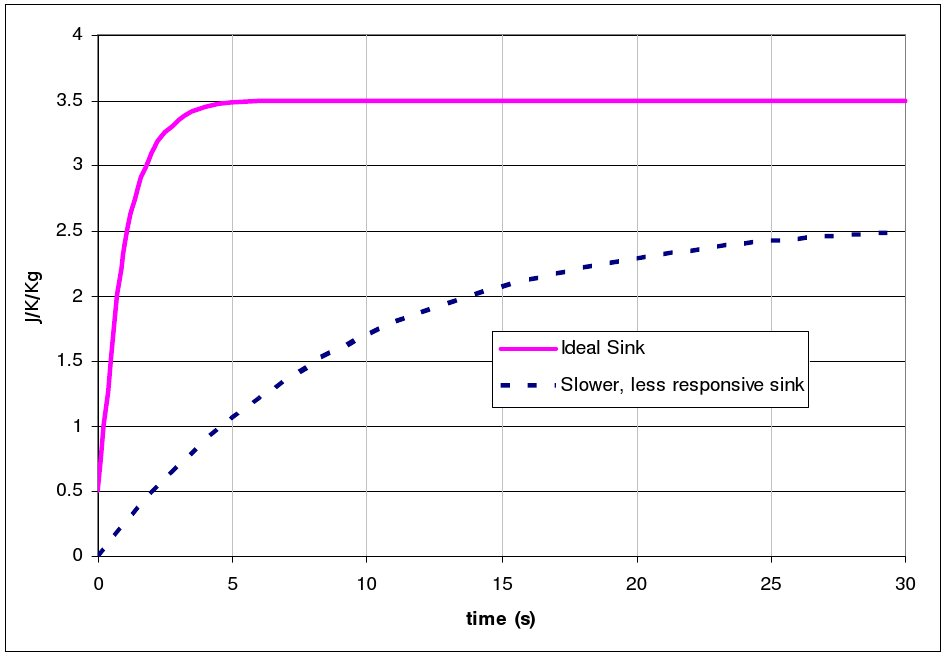
\includegraphics[scale=0.5]{sinkComp1.jpg}
 \caption[Theoretical Heat Sink Performances]{\textbf{\emph{Comparison plot of an ideal and low performance heat sink}} This model illustrates two materials of varying specific heat and thermal conductivity sinking thermal energy.\label{sinkComp1}}
\end{figure}

In this comparison, it's most important to note that no single parameter can summarize the complete thermal sink performance of a particular aggregate.

\subsection{Interpreting the Scaled, Normalized CET Function}
In graphically comparing different materials' trials with one another, the Scaled Normalized Cumulative Energy Transfer (CET) Function (SNCET) (Eq \ref{SNSCF}) was scaled by the measured heat capacity of the respective trial to yield a function with dimensions J/K/kg. This is a function that graphically illustrates the rate at which energy was exchanged with an amplitude that is analogous to the net energy transferred between water and aggregate. 
\begin{equation}\label{SNCSF}
 SNCET(t)\;=\;\dfrac{\Delta T(t)[TB]}{\sum\Delta T(t)[TB]}(c_{R})
\end{equation}
The primary purpose of creating a SNCET plot is to rank or compare different aggregate trials. It is a way to visualize and compare thermal sink performance amongst other aggregate families. Plots of the actual energy exchanged are listed in Appendix C, series 2. Shown is a SNCET plot of all medium flows in Figure (\ref{med1}). This plot serves to partially demonstrate the dominance of material over cobble size, noting how both SB1 (steel balls) and GB1 (glass balls) are 1'' in diameter with nearly identical characteristic radii. In aggregate trials, a comparable change in characteristic radius does not yield equally as dramatic differences in the SNCET plot. Additionally, noting how the aggregate materials have similar specific heats compared to SB1 and GB1, the most variance is a result of cobble size. 

In Figures \ref{med1} and \ref{low1}, each plot features several Scaled, Normalized Cumulative Energy Transfer (SNCET). Drawing from the aforementioned model in Figure \ref{sinkComp1}, several specific thermal sink characteristics can be interpreted. The rate of the function's rise to its maximum asymptote can be visually interpreted as the rate at which thermal energy is transferred into the aggregate mass, otherwise realized as the thermal conductivity. The value of the maximum asyptote is directly attributable to the heat capcity of the aggregate. As is argued with the thermal moment, $T_m$, both parameters need to be considered in rating a particular thermal sink performance. Generally, for maximum mitigation in an application, a large heat capcity is needed, but also at least a moderate to high thermal conductivity. The aggregates that offer the most promising SNCET are QM1 and QM6. 

\begin{landscape}
\begin{figure}
\vspace{4mm}
 \centering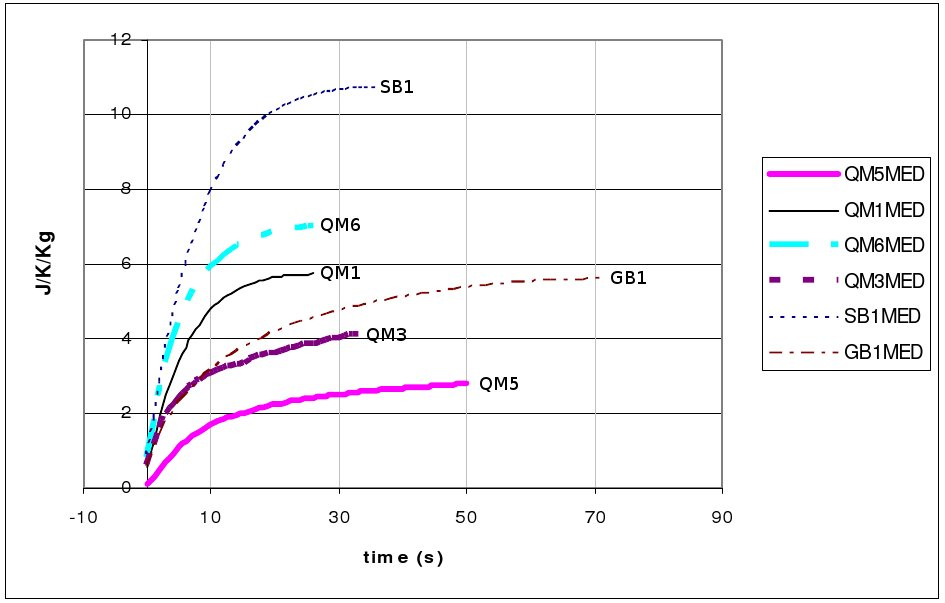
\includegraphics[scale=0.7]{med1.JPG}
 \caption[Scaled, Normalized CET - Medium Flow]{\textbf{\emph{Scaled, Normalized Cumulative Energy Transfer Function from medium rate trials}} Each trial is comparable in both a rate and quantity of thermal energy transfer under a medium flow rate.\label{med1}}
\end{figure}
\end{landscape}
\begin{landscape}
\begin{figure}
\vspace{4mm}
 \centering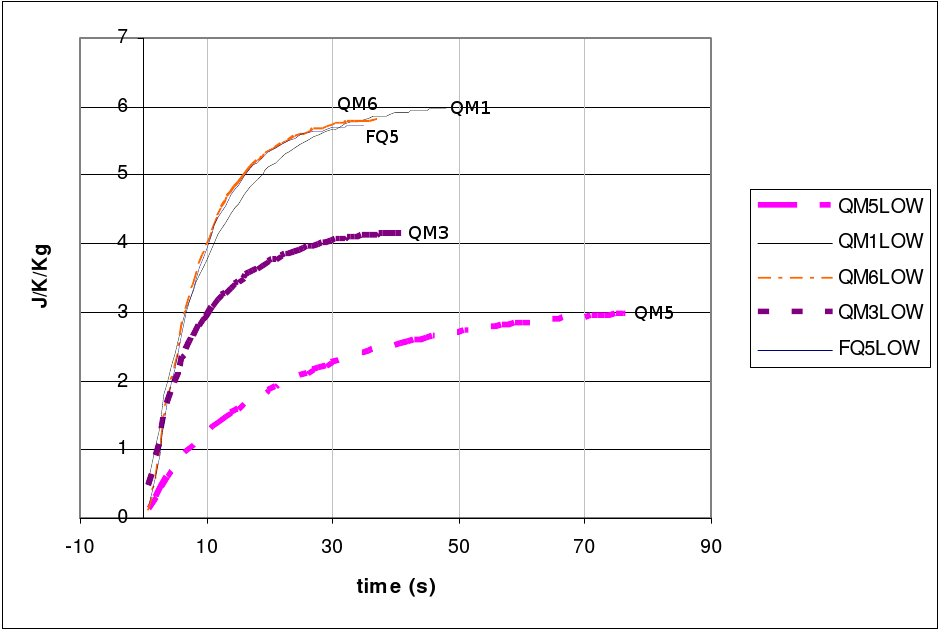
\includegraphics[scale=0.7]{low1.jpg}
 \caption[Scaled, Normalized CET - Low Flow]{\textbf{\emph{Scaled, Normalized Cumulative Energy Transfer Function from low rate trials}} Each trial is comparable in both a rate and quantity of thermal energy transfer under a low flow rate.\label{low1}}
\end{figure}
\end{landscape}
In Figure (\ref{med1}) two samples, QM.3 and QM5 offer thermal sink performances less than the glass balls. Each of these samples represent the extreme cobble sizes used in the experiments at 0.375'' and 5'', respectively. Noting how the mid-range cobble sizes offer both faster sink rates and total energy transferred during the trial, Figure (\ref{opt1}) demonstrates that there is an optimal cobble size for a given set of flow conditions. Note that this plot uses a maximum SNSCF value, so that this is actually expressing the total amount of energy that was transferred for a normalized temperature difference. Two different flows are depicted in Figures (\ref{med1}) and (\ref{low1}) - a medium and a low flow rate, for comparison. The flow rate seems to be a secondary parameter that stands to increase or decrease the amplitude of the curve while the cobble size will shift the peak of the curve left or right. 

\begin{figure}[h!]
\centering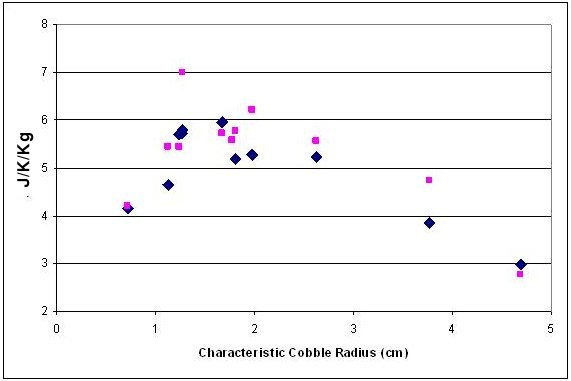
\includegraphics[scale=0.6]{opt2.JPG}
\caption[Scaled, Normalized CET vs Cobble Size]{\textbf{\emph{SNCET (J/K/Kg) versus cobble size - }} This plot shows an optimal cobble size under certain flow conditions. A low flow rate is represented by the diamond symbols, and a medium flow rate is represented by the squares.\label{opt1}}
\end{figure}

In studying this trend, the data indicate that as the flow rate increases, the optimal cobble size for thermal sink response should decrease slightly. This is intuitive, knowing that the larger cobbles possess a slower thermal response due to their bulk, and a lower flow can accomodate this best. A higher flow rate - and in turn a higher thermal wattage imparted on the aggregate -  will demand a faster thermal response than a smaller cobble could provide. There are, however, flow considerations to bear in mind as well, noting that a decrease in cobble size restricts flow, so in turn there is an optimization boundary. 

Hybrid aggregates warrant testing based on these results. It is conceivable that an aggregate of two or more different cobble sizes could offer both flow and thermal sink capacity with some compromise in total bulk. A preliminary analysis of a thermal sink capacity of such a material could be formulated from the current data. However, flow mechanics, the packing ratio and thermal contact parameters will naturally be different with hybrid aggregate, and so the exact results are not directly predictable from the current data.

\subsection{Thermal Conductivity, Moment and Diffusivity as Performance Indicators}
Thermal conductivity $\kappa$ is an intrinsic characteristic directly related to the material of the aggregate. It simply conveys the rate at which heat is transferred through the material, and it is the usual proportionality constant in modeling thermal energy transfers with the heat Equation. Thermal conductivity, as discussed in the experimentation section, is calculated from the data sets and then used to arrive at the thermal diffusivity. A high specific heat, sufficiently large cobble size and high thermal conductivity will help ensure that the aggregate can afford to remove more heat per unit time. 

The thermal moment, previously defined as $T_{m}=\frac{\kappa}{c_{R}}$, demonstrates that it is an important characteristic in the modelling of an aggregate's thermal response. In the experimental calculations, cobble size was embedded in the thermal conductivity as the gradient length, and therefore cobble size is inherent in the $\kappa$ values listed in this experiment. Ideally, $\kappa$ should compute to be the equal across the same material, but initial numerical calculations demonstrate a significant variance. This indicates that the cobbles are thermally loaded faster than the $\kappa$ calculations are assuming. According to Clauser \citep{kRocks}, quartzite has $k=7.7$ and the average for all quartzite cobble sizes used in experimentation is $k=10.5$. 

Thermal diffusivity is a quantitative measure for a particular mass's ability to respond to a thermal change in its environment. The lower the thermal diffusivity, the less thermal response per unit mass the sample will have. Diffusivity was computed in an attempt to arrive at some bulk unitary index with which to rate an aggregate, independent of flow. It is computed using bulk density and, of course, bulk temperature differentials, and so it should reflect the response of the entire aggregate mass as a whole. This is said with the assumption that a mass of aggregate will behave differently under duress when compared to a single cobble or material isolate.

%\paragraph{Power Analyses of Thermal Sink Capacity on a Themally Charged Creekflow}

%Optimally, $1-m^{3}$ of 1'' aggregate can produce up to 1000-kW of thermal sink power. A medium sized creek during a rain %event can be estimated at 3000-5000-kW at a peak flow rate of about $3-m^{3}$. 

\subsection{Recommendations for Thermal Buffering of Watersheds}

Temperature Total Maximum Daily Load (TMDL) regulations are imposed at both federal and state levels in select or sensitive waters that are subject to thermal charging from development, urban surfaces or industry \citep{urban}. Using construction aggregate for thermal buffering is only suitable where a small amount of energy needs to be removed from the flow. This could either be manifested as a short but dramatic rise in temperature levels from a point source or tributary or a small temperature change over a more prolonged period of time. The scope of this experiment was an investigation of point source mitgation under severe thermal duress for short periods of time. It is not reasonable to extrapolate these results to   time frames of more than a few minutes, especially if the aggregate is not enclosed. Convective and radiative heat loss will stand to yield much different thermal sinking effects if temperature differences are small and time frames are long.

Engineering solutions that currently implement aggregate as a thermal buffer typically lay the aggregate out in a piled mass to fill an entrenchment or drainaige basin that catches discharge before it is released into the watershed. In such scenarios, it can be stated that if there is known thermal spiking in the discharge, the aggregate will remove some thermal energy. However, analytically, flow patterns in piled gravel are not optimal for thermal sinking. In implementing an aggregate thermal sink, the following generalizations have been derived from the data:

\begin{itemize}
 \item Use of a medium sized cobble is preferred to allow sufficient flow, a minimum maintenance schedule and maximum thermal sink effects. These studies suggest $R_s=1-3\;cm$ for the flow rates measured.
 \item Arrangement of the aggregate such that the flow contacts as much of the available surface area as possible: Shallow surface arrangements, aggregate filled pipes or culverts, and baffles or flow vanes to redistribute the flow to other parts of the aggregate are all measures that could be taken to ensure maximal thermal contact area under flow.
 \item If a known point source exhibits thermal charging and its total thermal overload can be estimated in terms of a net energy difference, then for every unit volume of water that needs to be reduced by 1 degree, approximately that same volume of aggregate should be implemented to sink the flow. This is based on the assumption that the temperature differences between the aggregate and the overloaded water are greater than about 10 degrees. 
 \item For every unit volume of aggregate used, the thermal response of the creek will be damped by a factor proportional to the thermal moment of the aggregate and equal to the exponent in Equation (\ref{solution}). A simple analysis of this result can be visualized in the thermal sink power of the aggregate. If a thermally charged flow ramps with a known increase in flow rate and temperature, the thermal sink power of an ideally situated aggregate can be subtracted from the change in the discharge power to yield a reduced thermal acceleration or damping of the temperature spike. It should be stated that this is only a reasonable expectation for thermal sinking as the volume of aggregate needed to literally reduce the effective temperature increase by a few degrees in a storm induced flow is on the order of $10^{3}-m^{3}$ for even a very small creek.
 \item The maximum thermal sink power observed for an entire trial period in a common aggregate was 4-kW. Based on flow rate and thermal overloading conditions, this maximum sink power can be considered only under graviationally charged flow with no pressure head and less than 50\% flow capacity of the aggregate. Total immersion in a flow will only reduce this thermal sink power. 
\end{itemize}

\subsection{Conclusion}
Ultimately, the emphasis on using aggregate to thermally sink a thermally charged flow is to only damp a rapid change in temperature. The net change in temperature can only be artificially managed by eliminating or reducing thermal charging at the source or infiltration. 

Aggregates act to store heat for later release - damping the thermal spikes inherent to point sources. The effectiveness of this process is dictated primarily by (i) material composition, (ii) size, (iii) total mass, and (iv) packing fraction. The governing thermal parameters of the aggregate materials available on construction sites all fall within a narrow range such that the ideal solution would likely be a mixture of different materials and sizes small enough to retain the heated water for cooling while large enough to allow flow under large rain events. In addition, closed aggregate solutions in thermal contact with the earth would likely improve the thermal sink performance of the aggregate. Engineering solutions would have to be designed based on anticipated flow rates, overall discharge volumes, availability of aggregates, and ease in clean-out maintenance. This study clearly shows that effective thermal buffering can be achieved with such designs for small mountain streams exposed to flashy thermal charging.